\chapter{Benchmarking Returns}
\label{chap:Benchmarking Returns}

\begin{center}
\begin{tabular}{p{0.06\linewidth} | p{0.88\linewidth}}
	\toprule
	\multicolumn{2}{l}{\textbf{LEARNING OUTCOMES}} \\
	\midrule
	a & calculate and compare money-weighted and time-weighted rates of return \\
	\midrule
	b & describe the choices and the implications of the different weighting methods used in index construction and management, and calculate, interpret, and explain the value and the returns of an index \\
	\bottomrule
\end{tabular}
\end{center}

\vspace{1.5em}

\begin{itemize}
	\item[] \textbf{Money-Weighted and Time-Weighted Rates of Return}
	\item[] \textbf{Index Definition and Calculation}
	      \begin{itemize}
			\item[] Price Return and Total Return Indexes
			\item[] Index Weightings
			\item[] Index Management
			\item[] Comparing Index Performance
	      \end{itemize}
\end{itemize}

\section{Money-Weighted and Time-Weighted Rates of Return}
\label{sec:Money-Weighted and Time-Weighted Rates of Return}
\begin{center}
\begin{tabular}{p{0.06\linewidth} | p{0.88\linewidth}}
	a & calculate and compare money-weighted and time-weighted rates of return \\
\end{tabular}
\end{center}

\textcolor{blue}{\textit{Cần phân biệt TWR (hiệu quả quản lý quỹ) và MWR (hiệu quả đầu tư thực tế của cá nhân chịu ảnh hưởng từ dòng tiền).}}

\subsection{Time-Weighted Rate of Return (TWR)}
	\label{subsec:Time-Weighted Rate of Return (TWR)}
The time-weighted rate of return measures the compounded rate of growth of an investment portfolio over a specified horizon. To eliminate the distorting effects of external cash flows (which the investment manager typically does not control), the total investment horizon is broken down into subperiods at each cash flow event. The returns for each subperiod are calculated and then geometrically linked:
\begin{equation}
	r_{\text{TW}} = \prod_{t=1}^{T} (1 + r_t) - 1
	\label{eq:twr_m3}
\end{equation}
Note that $r_{\text{TW}}$ gauges a return for the whole time of all subperiod. 
If you want to estimate a mean return for \textbf{each} subperiod, you have to use $r_{\text{G}}$ 
\begin{equation}
	r_{\text{G}} = \sqrt[T]{\prod_{t=1}^{T} (1 + r_t)} - 1
	\label{eq:twr_G}
\end{equation}
% Reference: CFA Curriculum 2027, Volume 1, Module 3, Page 86

Where:
\begin{itemize}
	\item[] $r_{\text{TW}}$ is the time-weighted rate of return.
	\item[] $T$ is the total number of subperiods.
	\item[] $r_t$ is the holding period return for subperiod $t$, calculated between two successive cash flow events.
\end{itemize}

Because TWR measures performance between periods and filters out investor-driven contributions or withdrawals, it is the standard metric used to evaluate the investment skill of public market fund managers.

\subsection{Money-Weighted Rate of Return (MWR)}
	\label{subsec:Money-Weighted Rate of Return (MWR)}
The money-weighted rate of return (or dollar-weighted rate of return) measures the internal rate of return (IRR) of the investment. It accounts for both the size and timing of all cash flows. The MWR is the discount rate that sets the net present value of all cash flows equal to zero:
\begin{equation}
	0 = \sum_{t=0}^{T} \frac{\text{CF}_t}{(1 + r_{\text{MW}})^t}
	\label{eq:mwr_m3}
\end{equation}
% Reference: CFA Curriculum 2027, Volume 1, Module 3, Page 87

Where:
\begin{itemize}
	\item[] $r_{\text{MW}}$ is the money-weighted rate of return.
	\item[] $\text{CF}_t$ is the net cash flow at time $t$.
\end{itemize}

\textcolor{blue}{\textit{Quy ước dấu dòng tiền: Đầu tư ban đầu/góp thêm mang dấu âm (--); cổ tức, rút vốn/giá trị cuối kỳ mang dấu dương (+). Sử dụng máy tính tài chính (chức năng CF) hoặc Excel để giải MWR.}}

\subsection{Case Study}
	\label{subsec:Case Study: MWR vs TWR}
\begin{tcolorbox}[
	colback=gray!5!white,
	colframe=black!15!white,
	boxrule=0.5pt,
	arc=3pt,
	title=\textbf{Case Study: MWR vs TWR},
	coltitle=black,
	colbacktitle=black!5!white,
	before skip=6pt,
	after skip=6pt,
	breakable
]
	\begin{center}
		\captionof{table}{Money-Weighted Return for a Dividend-Paying Stock}
		% \label{tab:ex1}
		\begin{tabular}{p{0.1\linewidth} | p{0.6\linewidth}}
			\toprule
			\textbf{Time} & \textbf{Outflows}                                            \\
			\midrule
			0             & USD200 to purchase the first share                           \\
			1             & USD225 to purchase the second share                          \\
			\midrule
			\midrule
			\textbf{Time} & \textbf{Inflows}                                            \\
			\midrule
			1             & USD5 dividend received from first share (and not reinvested) \\
			2             & USD10 dividend (USD5 per share $\times$ 2 shares) received   \\
			2             & USD470 received from selling two shares at USD235 per share  \\
			\bottomrule
		\end{tabular}
	\end{center}
\begin{align*}
	& \Rightarrow CF_0 = -200 \qquad CF_1 = -220 \qquad CF_2 = +480 \\
	& \Rightarrow \frac{CF_0}{(1+IRR)^0} + \frac{CF_1}{(1+IRR)^1} + \frac{CF_2}{(1+IRR)^2}
	= \frac{-200}{1} + \frac{-220}{(1+IRR)^1} + \frac{+480}{(1+IRR)^2} \\
	& \Rightarrow IRR = 9.39\%
\end{align*}
Importantly, two investors in the same mutual fund or with the same portfolio of underlying investments may have different money-weighted returns because they invested different amounts in different years.

% \textcolor{blue}{\textit{Dòng tiền Albright: $\text{CF}_0 = -100$tr; $\text{CF}_1 = -30$tr (gồm $-20$tr góp thêm và $-10$tr tái đầu tư lãi vốn; cổ tức $2$tr tái đầu tư nên triệt tiêu); $\text{CF}_2 = 0$; $\text{CF}_3 = +140$tr (gồm giá trị cuối 137tr và 3tr cổ tức rút ra).}}

\begin{examtip}
	\textbf{Texas Instruments BA II Plus Keystrokes for MWR:}
	\begin{enumerate}
		\item Press \textbf{[CF]} $\rightarrow$ \textbf{[2nd]} \textbf{[CE|C]} $\rightarrow$ \textbf{[CLR WRK]} to clear worksheet memory.
		\item Enter $\text{CF}_0 = -200$: Press \textbf{200} $\rightarrow$ \textbf{[+/-]} $\rightarrow$ \textbf{[ENTER]}.
		\item Press \textbf{[$\downarrow$]} to display \textbf{C01}.
		\item Enter $\text{CF}_1 = -220$: Press \textbf{220} $\rightarrow$ \textbf{[+/-]} $\rightarrow$ \textbf{[ENTER]}.
		\item Press \textbf{[$\downarrow$]} $\rightarrow$ \textbf{[$\downarrow$]} to display \textbf{C02} (F01 defaults to 1).
		\item Enter $\text{CF}_2 = 480$: Press \textbf{480} $\rightarrow$ \textbf{[ENTER]}.
		% \item Press \textbf{[$\downarrow$]} $\rightarrow$ \textbf{[$\downarrow$]} to display \textbf{C03} (F02 defaults to 1).
		% \item Enter $\text{CF}_3 = 140$: Press \textbf{140} $\rightarrow$ \textbf{[ENTER]}.
		\item Press \textbf{[IRR]} then \textbf{[CPT]}.
	\end{enumerate}
\end{examtip}

\textcolor{blue}{\textit{
$HPR_1 = 15\%, HPR_2 = 6.7\%$, trong khi đó $MWR = IRR = 9.39\%, TWR = 10.76\%$. Bằng một ước tính gần đúng, ta có: (bạn có thể tự tính lại để kiểm tra)
\begin{align*}
	TWR & \approx \frac{HPR_1 + HPR_2}{2}\\
	MWR & \approx \frac{|CF_1|\cdot HPR_1 + |CF_2|\cdot HPR_2}{|CF_1|+|CF_2|}
\end{align*}
}}
\textcolor{blue}{\textit{Như vậy, dựa trên quan sát kết quả, ta nhận thấy, lợi suất của tài sản trong kỳ đầu tiên là cao hơn tương đối so với kỳ thứ hai ($HPR_1 > HPR_2$).\\
Dựa trên công thức xấp xỉ ở trên, ta có nhận xét rằng lợi suất bình quân tính theo MWR sẽ có trọng số dồn vào kỳ thứ hai nhiều hơn (do có dòng tiền phát sinh lớn hơn $|CF_2| > |CF_1|$, ở đây ta chỉ xét về độ lớn của dòng tiền, không xét về dấu).
Vậy nên, có thể hiểu rằng, dòng tiền lớn hơn đang dồn về kỳ có lợi suất thấp, nên nhìn chung sẽ hạ mức lợi suất trung bình xuống (vì vậy mà mức lợi suất này có tên gọi là money-weighted).\\
Còn nếu sử dụng TWR, ta coi mức lợi suất bình quân tính theo lợi suất từng kỳ với tỷ trọng như nhau, mà không phụ thuộc vào hiệu ứng dòng tiền đổ vào mỗi kỳ nhiều hay ít.
}}
\end{tcolorbox}

\subsection{Summary of Differences}
	\label{subsec:Summary of Differences}
Table \ref{tab:mwr_vs_twr_differences} summarizes the key comparisons between the two return methodologies.

\begin{table}[!htbp]
\centering
\caption{Comparison of Money-Weighted and Time-Weighted Returns}
\label{tab:mwr_vs_twr_differences}
\begin{tabular}{p{0.2\linewidth} p{0.35\linewidth} p{0.35\linewidth}}
\toprule
\textbf{Dimension} & \textbf{Money-Weighted Return (MWR)} & \textbf{Time-Weighted Return (TWR)} \\
\midrule
\textbf{Core Objective} & Measures the actual growth rate of the investor's funds. & Measures the compound growth rate of the portfolio assets. \\
\textbf{Cash Flow Sensitivity} & Highly sensitive to the size and timing of external cash flows. & Completely unaffected by external cash flows. \\
\textbf{Calculation Base} & Internal Rate of Return (IRR) equation. & Geometric linkage of subperiod returns. \\
\textbf{Performance Bias} & Can misrepresent manager skill if they cannot control cash flow timings. & Provides an objective measure of the manager's investment selection skill. \\
\textbf{Primary Suitability} & Recommended for private equity (where managers call capital) and individual investors. & Mandated by GIPS for public market mutual funds and active asset managers. \\
\bottomrule
\end{tabular}
\end{table}
% Reference: CFA Curriculum 2027, Volume 1, Module 3, Page 94

\section{Index Definition and Calculation}
\label{sec:Index Definition and Calculation}
\begin{center}
\begin{tabular}{p{0.06\linewidth} | p{0.88\linewidth}}
	b & describe the choices and the implications of the different weighting methods used in index construction and management, and calculate, interpret, and explain the value and the returns of an index \\
\end{tabular}
\end{center}

\textcolor{blue}{\textit{Market Index làm Benchmark và cơ sở cho ETF. Khi thiết kế chỉ số, cần lưu ý: (1) Cách tính (Price/Total Return) và (2) Phương pháp phân bổ tỷ trọng (Weighting Scheme).}}

\begin{examtip}[title={Cập nhật chương trình 2027}, colframe=red!75!black, colback=red!5!white]
Toàn bộ phần "Index Definition and Calculation" (xây dựng, quản lý chỉ số, các phương pháp trọng số giá/vốn hóa và tái cơ cấu danh mục chỉ số) là nội dung hoàn toàn mới được đưa vào cấu phần Quantitative Methods năm 2027. Trước đây nội dung này nằm ở các môn học khác (như Portfolio Management hay Equity).
\end{examtip}
\textcolor{blue}{\textit{Cụ thể về phân loại, nền tảng toán học và quy trình tính toán chỉ số, xem thêm tại Appendix \ref{chap:Index Definition and Calculation} (Index Definition and Calculation).}}

\begin{figure}[!htbp]
	\centering
	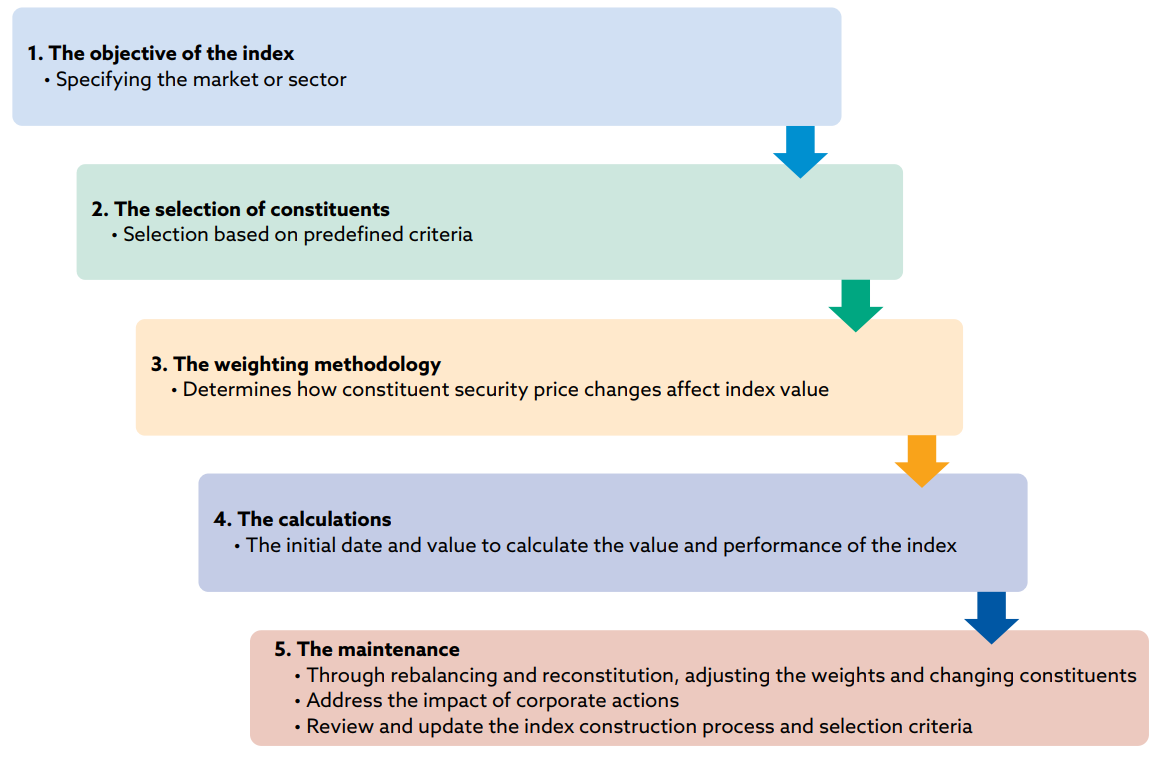
\includegraphics[width=0.85\linewidth]{002_figs/003_Module_3/exhibit_6.png}
	\caption{Steps in the Index Construction, Calculation, and Management Process}
	\label{fig:mod3_exhibit_6}
\end{figure}

\subsection{Price Return vs. Total Return Indexes}
	\label{subsec:Price Return vs. Total Return Indexes}
\begin{itemize}
	\item \textbf{Price Return Index ($r_{\text{PR}}$):} reflects only the prices of the constituent securities and measures capital appreciation:
	      \begin{equation}
		      r_{\text{PR}} = \frac{P_{t+1}}{P_t} - 1
		      \label{eq:price_return_rate}
	      \end{equation}
	      % Reference: CFA Curriculum 2027, Volume 1, Module 3, Page 99
	\item \textbf{Total Return Index ($r_{\text{TR}}$):} reflects both the prices and the reinvestment of all capital distributions (dividends/interest):
	      \begin{equation}
		      r_{\text{TR}} = \frac{P_{t+1} + \text{Div}_{t+1}}{P_t} - 1
		      \label{eq:total_return_rate}
	      \end{equation}
	      % Reference: CFA Curriculum 2027, Volume 1, Module 3, Page 99
\end{itemize}
Over time, the total return index will significantly outperform the price return index due to the compounding effect of reinvested cash distributions.

% \begin{figure}[!htbp]
% 	\centering
% 	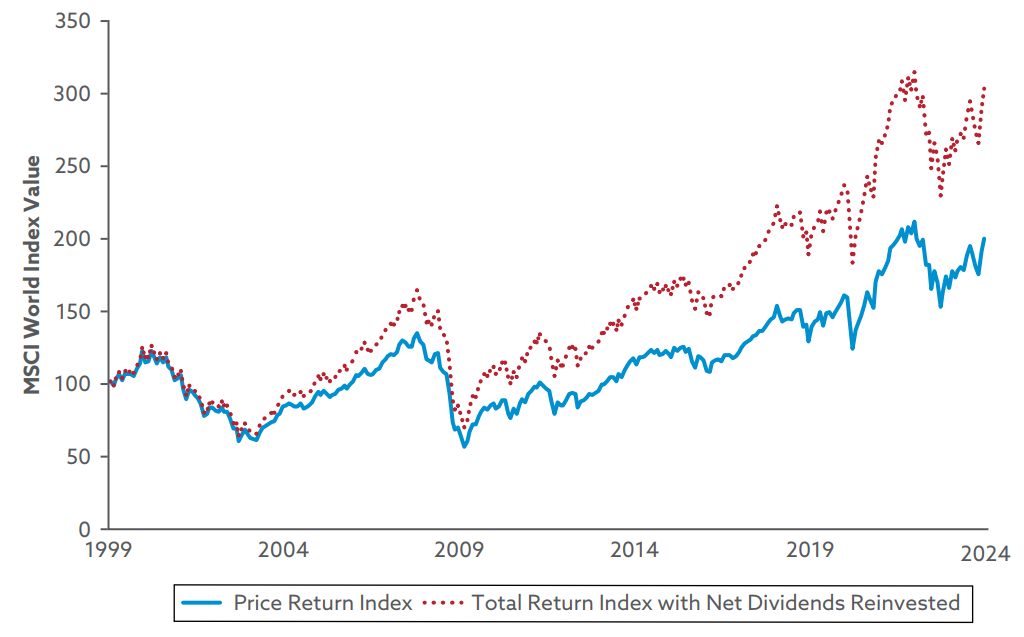
\includegraphics[width=0.85\linewidth]{002_figs/003_Module_3/exhibit_7.png}
% 	\caption{MSCI World Index Price Return vs. Total Return (1999--2023)}
% 	\label{fig:msci_world_price_vs_total}
% \end{figure}
% Reference: CFA Curriculum 2027, Volume 1, Module 3, Page 100

\textcolor{blue}{\textit{Công thức liên kết giá trị chỉ số Price Return và Total Return qua nhiều thời kỳ (kèm cơ chế tái đầu tư cổ tức và giá điều chỉnh Adjusted Price), xem thêm chi tiết tại phần (\ref{sec:app_index_return}).}}

\subsection{Index Weighting Methodologies}
	\label{subsec:Index Weighting Methodologies}
The general formula for calculating an index value at time $t$ is:
\begin{equation}
	\text{Index Value}_t = \sum_{i=1}^{N} w_{i,t} \times P_{i,t}
	\label{eq:general_index_value}
\end{equation}
% Reference: CFA Curriculum 2027, Volume 1, Module 3, Page 100

Where:
\begin{itemize}
	\item[] $w_{i,t}$ is the weight of constituent $i$ at time $t$.
	\item[] $P_{i,t}$ is the price of constituent $i$ at time $t$.
\end{itemize}

Let's review the five primary weighting methodologies:
\begin{enumerate}
	\item \textbf{Market Capitalization Weighting:} Weights are proportional to the total market capitalization ($Q_i P_i$):
	      \begin{equation}
		      w_i^M = \frac{Q_i P_i}{\sum_{j=1}^{N} Q_j P_j}
		      \label{eq:market_cap_weight}
	      \end{equation}
	      % Reference: CFA Curriculum 2027, Volume 1, Module 3, Page 101
	      The index value is often calculated using a divisor ($D_t$) to normalize the value:
	      \begin{equation}
		      V_t = \frac{\sum_{i=1}^{N} Q_{i,t} P_{i,t}}{D_t}
		      \label{eq:divisor_index_value}
	      \end{equation}
	      % Reference: CFA Curriculum 2027, Volume 1, Module 3, Page 101

	\item \textbf{Float-Adjusted Market Cap Weighting:} Accounts only for shares available to the public ($f_i Q_i$), excluding strategic holdings:
	      \begin{equation}
		      w_i^{M,\text{Float}} = \frac{f_i Q_i P_i}{\sum_{j=1}^{N} f_j Q_j P_j}
		      \label{eq:float_adjusted_weight}
	      \end{equation}
	      % Reference: CFA Curriculum 2027, Volume 1, Module 3, Page 104

	\item \textbf{Fundamental Weighting:} Weights are based on economic or accounting indicators (e.g., book value, revenues, earnings, or dividends) instead of market prices:
	      \begin{equation}
		      w_i^F = \frac{F_i}{\sum_{j=1}^{N} F_j}
		      \label{eq:fundamental_weight}
	      \end{equation}
	      % Reference: CFA Curriculum 2027, Volume 1, Module 3, Page 109

	\item \textbf{Price Weighting:} Weights are proportional to the security price per share:
	      \begin{equation}
		      w_i^P = \frac{P_i}{\sum_{j=1}^{N} P_j}
		      \label{eq:price_weight}
	      \end{equation}
	      % Reference: CFA Curriculum 2027, Volume 1, Module 3, Page 109
	      The index value is calculated by dividing the sum of constituent prices by a divisor ($D_t$):
	      \begin{equation}
		      V_{\text{PRI},t} = \frac{\sum_{i=1}^{N} P_{i,t}}{D_t}
		      \label{eq:price_weighted_value}
	      \end{equation}
	      % Reference: CFA Curriculum 2027, Volume 1, Module 3, Page 109

	\item \textbf{Equal Weighting:} Each security is assigned an equal share at the inception/rebalancing date:
	      \begin{equation}
		      w_i^E = \frac{1}{N}
		      \label{eq:equal_weight}
	      \end{equation}
	      % Reference: CFA Curriculum 2027, Volume 1, Module 3, Page 111
	      The index value is:
	      \begin{equation}
		      V_{\text{EQI},t} = \frac{\sum_{i=1}^{N} n_i P_{i,t}}{D_t}
		      \label{eq:equal_weighted_value}
	      \end{equation}
	      % Reference: CFA Curriculum 2027, Volume 1, Module 3, Page 111
\end{enumerate}

\subsection{Summary of Weighting Methodologies}
	\label{subsec:Summary of Weighting Methodologies}
Table \ref{tab:index_weighting_methodologies_summary} compares the characteristics of these methodologies.

\begin{table}[!htbp]
\centering
\caption{Comparison of Index-Weighting Methodologies}
\label{tab:index_weighting_methodologies_summary}
\begin{tabular}{p{0.15\linewidth} p{0.15\linewidth} p{0.15\linewidth} p{0.2\linewidth} p{0.2\linewidth}}
\toprule
\textbf{Index Type} & \textbf{Weighting Basis} & \textbf{Examples} & \textbf{Pros} & \textbf{Cons} \\
\midrule
\textbf{Market Cap} & Proportional to market capitalization. & S\&P 500, MSCI World, S\&P BSE SENSEX & Reflects relative sizes; low turnover; automatic rebalancing. & Concentrated in top firms; overweights overpriced stocks. \\
\midrule
\textbf{Equal Weighted} & Identical weight ($1/N$). & S\&P 500 Equal Weight, MSCI USA Equal Weight & Reduces concentration risk; enhances exposure to smaller firms. & Requires frequent rebalancing; high turnover and transaction costs. \\
\midrule
\textbf{Fundamental} & Economic metrics (sales, dividends, book value). & FTSE RAFI US 1000 & Focuses on firm size over market sentiment; value bias. & Sector bias; excludes firms with zero earnings or dividends. \\
\midrule
\textbf{Price Weighted} & Share price ($P_i$). & Dow Jones Industrial Average (DJIA), Nikkei 225 & Simple to calculate and interpret. & High price stocks dominate index; stock splits distort weights. \\
\bottomrule
\end{tabular}
\end{table}
% Reference: CFA Curriculum 2027, Volume 1, Module 3, Page 102

\textcolor{blue}{\textit{Chỉ số vốn hóa tự điều chỉnh tỷ trọng (Self-Rebalancing), giúp giảm chi phí giao dịch. Tuy nhiên, nó bị ảnh hưởng bởi đà tăng giá (momentum bias), ép mua nhiều các cổ phiếu đang bị định giá quá cao.}}

\textcolor{blue}{\textit{Chi tiết cách xác định số lượng cổ phiếu giả định ($n_i$) và quy mô danh nghĩa ($A_r$) cho từng phương pháp phân bổ tỷ trọng (Market Cap, Float-Adjusted, Fundamental, Price, Equal), xem thêm phần (\ref{sec:app_index_weights}) và (\ref{sec:app_index_constituent_shares}).}}

\subsection{Index Management: Rebalancing and Reconstitution}
	\label{subsec:Index Management: Rebalancing and Reconstitution}
\begin{itemize}
	\item \textbf{Periodic Rebalancing:} adjusts the weights of the constituents back to their target levels. This is critical for equal-weighted and fundamentally weighted indexes because price variations cause weights to drift. Equal-weighted indexes require counter-trend trading (selling winners and buying losers), which increases transaction costs and portfolio turnover.
	\item \textbf{Reconstitution:} the periodic process of adding or removing constituent securities from the index based on eligibility rules. Widely followed indexes often apply a \textit{banding strategy} (e.g., Russell 2000's 5\% band) to reduce unnecessary index turnover at the breakpoints.
\end{itemize}

\textcolor{blue}{\textit{Công thức toán học mô tả sự lệch tỷ trọng thực tế ($w_{i,t}^{\text{actual}}$) và cơ chế điều chỉnh Divisor mới ($D^+$) khi thay đổi danh mục (Reconstitution), xem thêm phần (\ref{sec:app_index_rebalance_reconstitution}).}}

% \begin{figure}[!htbp]
% 	\centering
% 	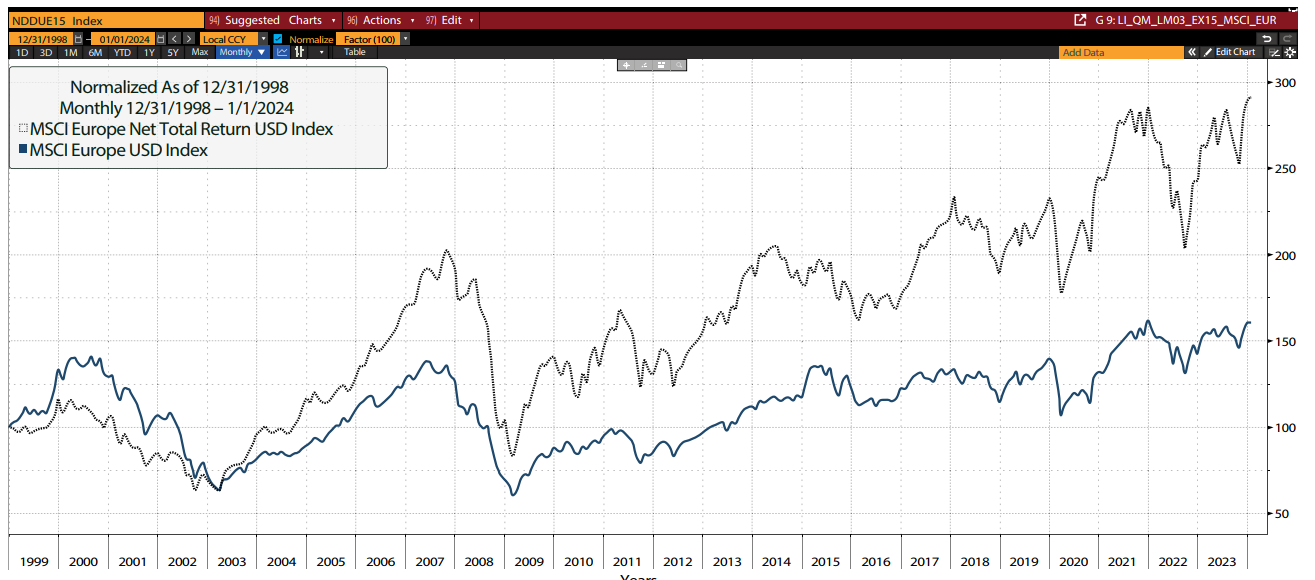
\includegraphics[width=0.85\linewidth]{002_figs/003_Module_3/exhibit_15.png}
% 	\caption{MSCI Europe Equal-Weighted vs. MSCI Europe Market Cap-Weighted (1999--2023)}
% 	\label{fig:msci_europe_equal_vs_cap}
% \end{figure}
% Reference: CFA Curriculum 2027, Volume 1, Module 3, Page 115

\subsection{Divisor Adjustment for Stock Splits}
	\label{subsec:Divisor Adjustment for Stock Splits}
In a price-weighted index, when a constituent stock splits, its price per share drops mechanically without any change in its actual economic value or the firm's market capitalization. To prevent the index value from dropping artificially, the divisor ($D$) must be adjusted downward:
\begin{equation}
	D_{\text{new}} = \frac{\sum P_{\text{new}}}{V_{\text{PRI, before}}}
	\label{eq:divisor_adjustment}
\end{equation}
% Reference: CFA Curriculum 2027, Volume 1, Module 3, Page 118

\begin{tcolorbox}[
	colback=gray!5!white,
	colframe=black!15!white,
	boxrule=0.5pt,
	arc=3pt,
	title=\textbf{Example: Divisor Adjustment for Stock Splits},
	coltitle=black,
	colbacktitle=black!5!white,
	before skip=6pt,
	after skip=6pt,
	breakable
]
Consider a price-weighted index with 5 stocks: A ($50$), B ($40$), C ($30$), D ($25$), E ($5$). Divisor $D_{\text{old}} = 1.5$.
\begin{itemize}
	\item \textbf{Before Split:} The index value is:
	      \[ V_{\text{PRI}} = \frac{50+40+30+25+5}{1.5} = 100 \]
	\item \textbf{After 2-for-1 Split of A:} Stock A's price drops from 50 to 25. The new price sum is $25+40+30+25+5 = 125$.
	\item \textbf{Divisor Adjustment:} To keep the index value unchanged at 100:
	      \[ D_{\text{new}} = \frac{125}{100} = 1.25 \]
\end{itemize}

\textcolor{blue}{\textit{Khi cổ phiếu chia tách làm giá giảm, Divisor phải giảm tương ứng để giữ điểm số chỉ số không bị thay đổi ảo.}}
\end{tcolorbox}

\textcolor{blue}{\textit{Xem thêm về nguyên lý tổng quát điều chỉnh Divisor ($D_t = D_{t-1} \times \frac{A_t^*}{A_{t-1}}$) và mô hình 4 lớp tư duy xây dựng chỉ số tại phần (\ref{sec:app_index_divisor}) và (\ref{sec:app_index_conclusion}).}}


% \section{Practice Problems and Solutions}
% \label{sec:Practice_Problems_Module_3}
% \textcolor{blue}{\textit{Các bài tập ôn tập kèm Lời giải của Module 3 đã được chuyển về Chương 14 (Bài tập ôn tập và Lời giải) ở cuối bản PDF để tiện tra cứu tập trung. Xem bài tập và lời giải tại trang \pageref{sec:app_Problems_M3}.}}
